\chapter*{Entracte: What the Hare Said to Patroclus}
\addcontentsline{toc}{chapter}{Entracte: What the Hare Said to Patroclus}
\renewcommand\thefigure{E.\arabic{figure}}
\setcounter{figure}{0}
\chaptermark{Entracte: What the Hare Said to Patroclus}
\markboth{Entracte: What the Hare Said to Patroclus}{Entracte: What the Hare Said to Patroclus}

\begin{marginfigure}[5.5cm]
	\centering
	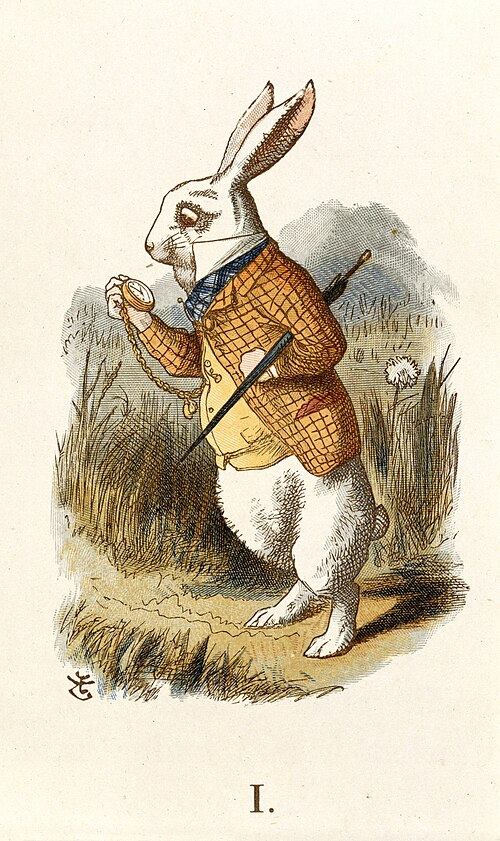
\includegraphics[width=\linewidth]{fig/WhiteRabbit.jpg}
	\caption{
		Overconfident, the Hare preferred to think
		about algebraic language theory rather than how to win the upcoming race,
		see \cite{Carroll1895TortoiseAchilles}.
		\href{https://commons.wikimedia.org/wiki/File:The\_White\_Rabbit\_\%28Tenniel\%29\_-\_The\_Nursery\_Alice\_\%281890\%29\_-\_BL.jpg\#/media/File:Alice\_par\_John\_Tenniel\_02.svg}{\emph{The White Rabbit}}, by John Tenniel.
	}
\end{marginfigure}
Waiting for Achilles to return from his race, Patroclus stumbled onto a Hare that appeared to be lost in deep thought.
\par ``Greetings, my friend. What seems to be bothering you?'' inquired the Greek.
\par ``Well, I have been thinking about Automedon---an automaton I mean'' answered the Hare, ``for I want to study rationality, but the notion of computation eludes me. After all, Babbage’s machine hasn't been invented yet!''
\par ``By far the most natural way of understanding rational languages is through the lens of algebra,'' Achilles’ lover explained. ``They simply consist of languages recognized by finite monoids.''
\par ``A monoid? What in Zeus's name is this?''
\par ``Are you familiar with category theory? It is a branch of mathematics---''
\par ``A branch of mathematics? What need do you have of having multiple branches? Have you found inconsistencies in Euclid’s axioms?'' interrupted the Hare.
\par ``Not exactly. It provides a useful framework to abstractly study different structures. In geometry, points are considered atomic objects, and they are connected through shapes. In category theory, points are abstracted, and shapes are treated as first-class citizens, connected by shape transformations.''
\par ``This seems rather pointless… But if such abstract nonsense is what you have to endure to have provably consistent foundations of mathematics, I suppose it might be worth it,'' conceded the Hare.
\par ``Anyway,'' added Patroclus after a brief pause, ``a monoid can simply be defined as an Eilenberg-Moore algebra for the monad of finite words in the category of sets.'' 
\par ``A monad? Don’t tell me that after disavowing points you abjured all gods but one.''
\par ``It has nothing to do with religion, put some faith in category theory: a monad is quite simple to define'' said Patroclus. ``Endofunctors of a category form themselves a category, whose morphisms are natural transformations. A monad consists of nothing else but a monoid in this category.''
\par ``A monoid? What in Zeus's name is this?'' echoed the Hare.

At this point, the narrator, having to write his thesis, had to leave our two protagonists to their discussion. Several days passed after he submitted his manuscript when he went back to the spot, only to find the two companions arguing.
\par ``As I said, a monad is a monoid in the category of endofunctors!'' Patroclus exclaimed, visibly irritated.
\par ``But that doesn’t help me understand what is a monoid…'' the exhausted Hare replied, ``at least we can hope for logicians not to be foolish enough to define rationality using monads.''
